                    %RELATÓRIO DO PROJETO DE SISTEMAS OPERATIVOS 2019 - Gestão de Vendas

%----------------------------------------------------------------------------------------------------------------------

\documentclass[a4paper,11pt]{report}
\usepackage[utf8]{inputenc}
\usepackage[portuguese]{babel}
\usepackage{graphicx}
\usepackage{hyperref}
\usepackage{float}
\usepackage{listings}


%----------------------------------------------------------------------------------------------------------------------

\usepackage{geometry}
 \geometry{
     a4paper,
     total={170mm,257mm},
     left=25mm,
     right=25mm,
     top=20mm,
 }

\graphicspath{{./base_images/}}

%----------------------------------------------------------------------------------------------------------------------

\begin{document}

%----------------------------------------------------------------------------------------------------------------------


\begin{titlepage}
    \center
    {

    \begin{figure}[t]
        \centering
        
\includegraphics[scale=0.4]{uminho.png}
        \label{img:logo}
        \vspace{2.0cm}
    \end{figure}

    \vspace{3.0cm}
    \textsc{\huge Sistemas Operativos}\\[0.5cm]
    \textsc{\Large{Mestrado Integrado em Engenharia Informática}}\\[0.5cm]
    \vspace{4.0cm}
    \textsc{\Huge{Gestão de Vendas}}\\[0.5cm]
    \vspace{5.0cm}
    \begin{flushleft}
        \vspace{2.0cm}

        \large A85227 \,\,\,João Pedro Rodrigues Azevedo
        \vspace{0.2cm}

        A85729 \,\,\,Paulo Jorge da Silva Araújo
        \vspace{0.2cm}

        A83719 \,\,\,Pedro Filipe da Costa Machado
    \end{flushleft}
        \vspace{1cm}
    \begin{flushright}
        Braga

        Maio 2019
    \end{flushright}

\date{\today}
}
\end{titlepage}

%----------------------------------------------------------------------------------------------------------------------

%Indice

\tableofcontents
\clearpage

%---------------------------------------------------------------------------------------------------------------------
%---------------------------------------------------------------------------------------------------------------------

% Introdução

\chapter{Introdução}

\hspace{0.50cm} Este trabalho foi realizado no âmbito da unidade curricular de Sistemas Operativos do curso de Mestrado Integrado em Engenharia Informática (MIEI). \par

\vspace{0.5cm}

Esta UC, assim como este trabalho prático, tinha como principal objetivo a utilização de conhecimentos Teóricos e 
Práticos relativos à manipulação de ficheiros, gestão de processos, memória e utilização de CPU pelas diferentes entidades que o consomem (Processos). 

\vspace{0.5cm}

Deste modo, foram importantes conhecimentos relativos ao escalonamento de processos, sincronização e também concorrência para a realização deste trabalho prático. \par

\section{Objectivos}

\hspace{0.50cm} Neste trabalho pretende-se construir um protótipo de um sistema de gestão de inventário e vendas. O
sistema deverá ser constituído por vários programas: manutenção de artigos, servidor de vendas, cliente
de vendas, e agregador de dados. \par 

\vspace{0.5cm}

A interação de possivéis clientes com os programas são comunicadas ao servidor que deverá controlar e garantir a correta resposta e segurança oferecida pelo mesmo de modo a escalonar o débito de dados e pedidos recebidos garantindo, portanto, uma resposta eficiente aos mesmos.

\section{Outros aspetos (Organização do projeto)}

\hspace{0.50cm} Este projeto possui uma organização lógica de pastas contendo cada uma um dos programas pedidos, dentro da pasta source "src/". \par
Na pasta "FILES/" encontram-se os ficheiros ARTIGOS, STRINGS, STOCKS e VENDAS pedidos (e outros, como por exemplo, registo de erros no decorrer dos programas) e na pasta "PipeVendas/" estarão armazenados os pipes de comunicação com o servidor e ficheiros com registos de clientes no sistema (e os seus PIDs) e também alguns registos importantes para o agregador.


%---------------------------------------------------------------------------------------------------------------------
%---------------------------------------------------------------------------------------------------------------------

\chapter{Descrição do projeto}

\hspace{0.50cm} Neste capítulo serão descritos os procedimentos, estratégias e todos os programas implementados bem como justificações sobre utilização de certas estruturas e ficheiros para o correto funcionamento de todo o sistema. \par
Além das operações pedidas são realizadas outras para permitir um melhor processo de \textit{debugging} e registo de clientes/pedidos:
 
\begin{itemize}
  \item Registo de erros (personalizados) relativos a comandos, números introduzidos, erros de leitura/escrita, etc...
  \item Registo de todos os clientes com \textit{log in} no sistema
  \item ...
\end{itemize}

\section{Manutenção de artigos}

\hspace{0.50cm} Este programa permite a introdução e modificação de produtos pertencentes ao sistema através de 3 comandos principais (e 1 secundário), sendo eles:

\begin{lstlisting}[language=bash]

    $ ma
    i <nome> <preco> (insere novo artigo, mostra o codigo)
    n <codigo> <novo nome> (altera nome do artigo)
    p <codigo> <novo preco> (altera preco do artigo)
    a (efetua a agregacao das VENDAS)
    ...
    <EOF>

\end{lstlisting}
    
Segue-se a descrição da organização dos ficheiros de dados ARTIGOS [22 bytes/linha], STOCKS [11 bytes/linha] E STRINGS [nº de bytes variáveis/linha]:

\begin{lstlisting}
    
    Codigo | <Referencia> <Preco> [ARTIGOS]
    Codigo | <Nome>               [STRINGS]
    Codigo | <qt_stock>           [STOCKS]
    
    1| 

\end{lstlisting}
   
Aqui o Codigo representa a linha no ficheiro [Codigo fixo do artigo], a referência representa a linha onde se encontra no ficheiro strings [Referencia variavel mas inicialmente igual ao codigo] e por fim o preço e quantidade de stock são propriedades do artigo.

É de realçar que os tamanhos fixos de todos os ficheiros (exceto o STRINGS) permitem uma leitura/escrita atómica através de \textit{system calls: read e write.} \par 
Nota: tal não acontece com o ficheiro de nomes o que implica a utilização de uma função que faz a leitura byte a byte de uma string input.

Em relação ao comando "a" é de referir que o pedido de agregação só é realizado se o servidor estiver \textit{online}, ou seja, em execução. Caso contrário o pedido será negado e uma mensagem de erro será impressa no STDERR do "ma".

\section{Servidor de vendas}

\hspace{0.50cm} Este é o \textit{core} do sistema de vendas, recebe pedidos de clientes através de um pipe comum a todos os clientes e envia respostas através de um pipe indiviual. Tal se processa utilizando o \textbf{Process ID} do cliente como sendo o seu identificador \textbf{único} que é enviado em conjunto com o seu pedido sendo a respetiva resposta enviada por um pipe por cliente. \par

Visto que o servidor responde a um conjunto de pedidos dos clientes, tal será importante ser explicitado primeiro, passemos a descrição para o \textbf{cliente de vendas}.

\vspace{1.5cm}

\begin{figure}[h]
    \centering
    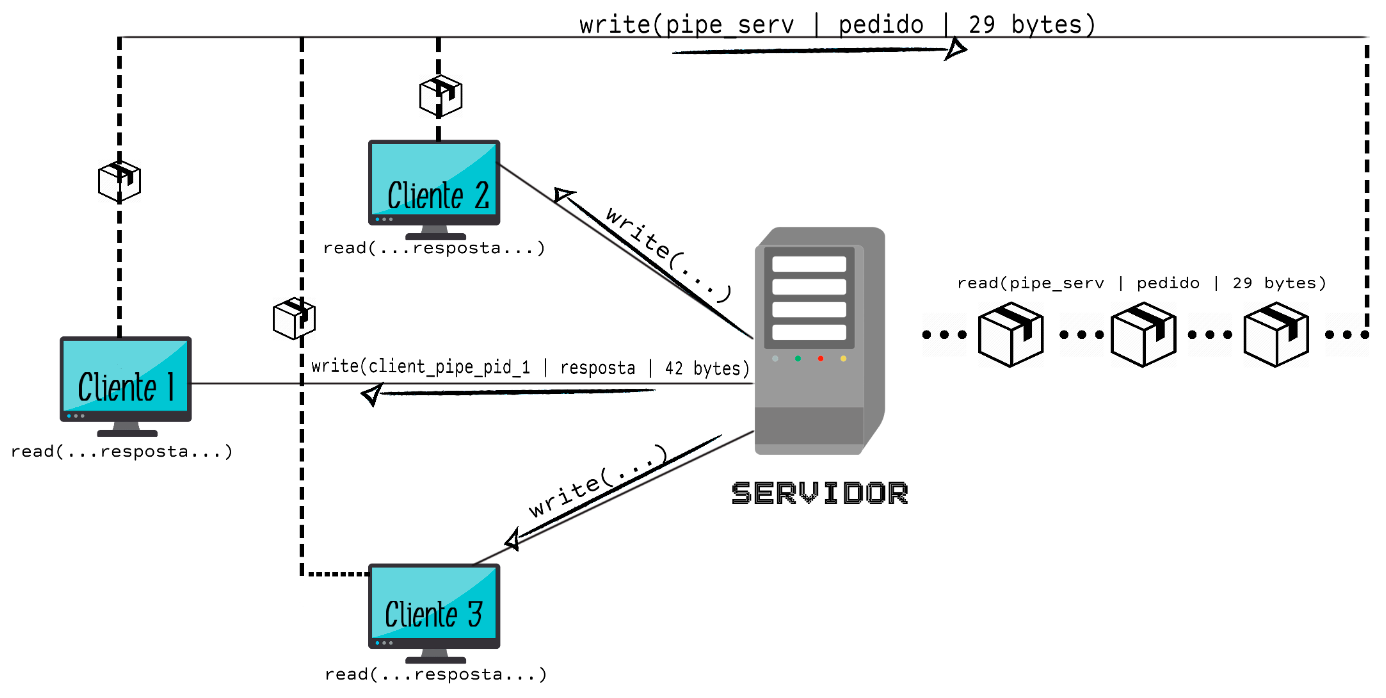
\includegraphics[scale=0.5]{cliente_server.png}
    \label{img:serverclient}
    \caption{Representação do sistema cliente-servidor.}
\end{figure}

\subsection{Cliente de Vendas - Comandos permitidos}

\hspace{0.50cm} Um cliente deste sistema de vendas tem a possibilidade de visualizar stock e preço de um artigo e também de alterar a quantidade de stock (aumentando ou diminuindo o mesmo), sendo que uma diminuição de stock implica um registo de uma venda. Segue-se a descrição dos comandos possiveis.

\begin{lstlisting}[language=bash]

$ cv
<codigo> (mostra no stdout stock e preco)
<codigo> <quantidade> (actualiza stock e mostra novo stock)
...
<EOF>

\end{lstlisting}
   
De forma geral, um cliente introduz comandos a partir do seu STDIN e recebe as repostas no seu STDOUT (formatadas de forma diferente dependendo do pedido).

\subsection{Pedidos e Respostas}
   
\hspace{0.50cm} Os pedidos são enviados para o servidor por um \textit{named pipe} (FIFO - \textit{first in first out}) e são processados, um a um. Eis alguns exemplos de \textit{buffers} contendo pedidos de clientes enviados ao servidor:
   
   
\begin{lstlisting}[language=C]
    
    //Codigo que gera o pedido
    sprintf(pedidoBuffer, "%07d %010d %010d", clientPID, codigo, quantidade);
    
    //Exemplo de pedido
    //PID CODIGO QUANT
    
\end{lstlisting}
   
   \vspace{0.5cm}
   
    Cada pedido tem um tamanho fixo de 29 bytes escritos e lidos atomicamente. Seguem-se exemplos de repostas do servidor:
   
\begin{lstlisting}[language=C]
    
    sprintf(bufferEscrita, "0 %07d %010d %010d %010d", clientID,         codigoProduto,  quantidadeStock, precoLido);
	
	//Aqui o primeiro byte, o "0", 
	// representa um dos tipos de resposta
	//Chegando ao cliente, mediante essa flag, 
	// este sabe que resposta apresentar.
										   
\end{lstlisting}

\vspace{1.0cm}

Cada resposta utiliza 42 bytes. Todas estas constantes, \textit{defines} e \textit{paths} estão presentes no ficheiro "global.h"\footnote{Source que contém uma coleção de funções auxiliares ao projeto e constantes importantes.} da diretoria GLOBAL-SOURCE.

\section{Agregador}

\hspace{0.50cm} O agregador utiliza os registos de vendas presentes no ficheiro VENDAS e coleciona vendas agregando a quantidade vendida e o montante (preco x quantidade comprada) numa mesma entrada de um novo ficheiro gerado (cujo nome é dado pela data:hora:min no momento de agregação).

A implementação passou pela criação de uma HashTable\footnote{São usadas estruturas otimizadas, GLib.}, cuja \textit{key} é o codigo do produto, após \textit{parsing} de uma venda e o respetivo value é composto pela quantidade comprada e montante de venda. \par

As entradas que têm \textit{hashing} para a mesma posição agregam-se num lista de registos de venda sendo posteriormente convertidas apenas numa venda (agregada). A imagem seguinte descreve a estrutura implementada:

\begin{figure}[H]
    \centering
    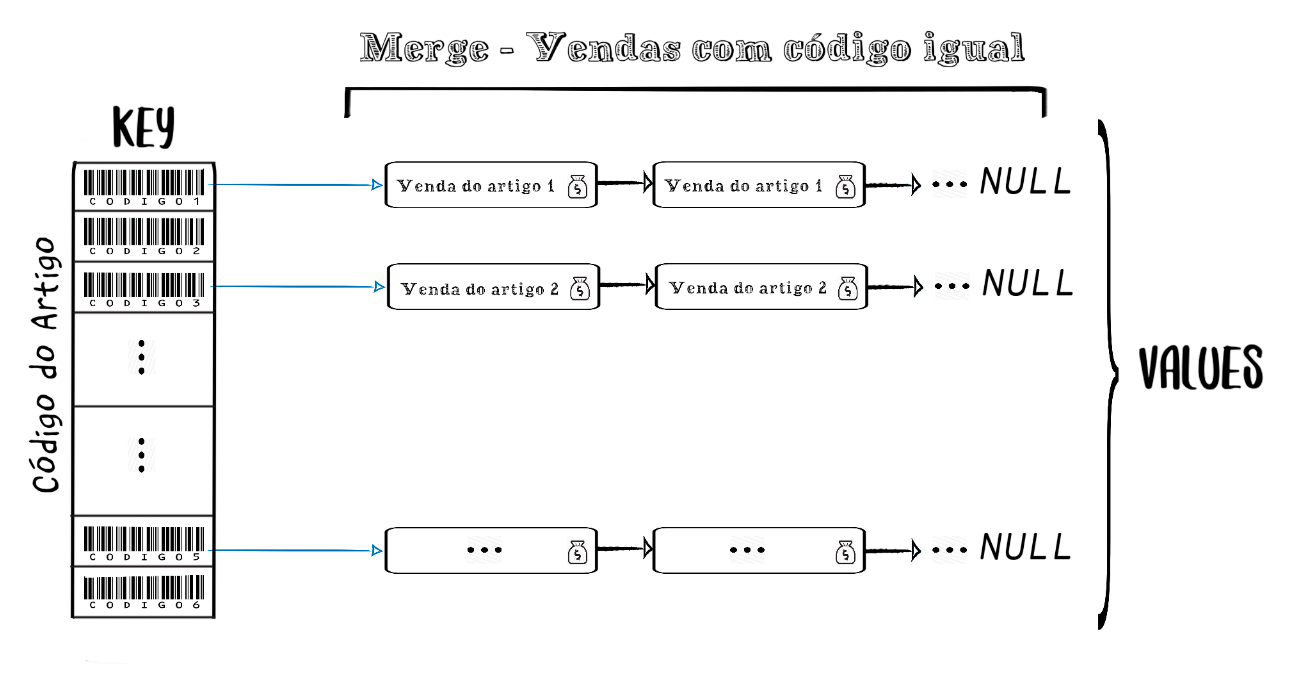
\includegraphics[scale=0.5]{htag.png}
    \label{img:htag}
    \caption{Estrutura utilizada no agregador.}
\end{figure}

A importância da criação desta HashTable passa pela procura de otimização do processo de agregação devido à sua procura constante \textit{O(1)}.

\subsection{Agregação concorrente}
\vspace{1.0cm}

\hspace{0.50cm} Para este tipo de agregação tem se em consideração a criação de processos que efetuam a agregação de partes do ficheiro VENDAS, divindo o trabalho de forma equivalente. Ora isto traz a noção de paralelismo ao projeto, apesar de que a execução não é necessariamente paralela (Devido à gestão de processos do Sistema Operativo) mas providencia um melhoramento de performance ao trabalho.
Mais à frente será descrita a implementação adotada.
\vspace{1.0cm}

Quanto à implementação a solução é simples, trata-se de arranjar uma forma de dividir trabalho e criar processos q.b. para agregar concorrentemente. O grupo decidiu estabelecer um limite inferior de linhas para criação de processos com  \textit{fork()} e, pela experiência, concluimos que 5000 seria um numero razoável devido aos testes que o programa poderá estar sujeito. 
\vspace{1.0cm}

Um exemplo muito custoso (testado inicialmente pelo grupo) seria colocar um limite de 1000...Num caso de termos 150 mil registos venda o programa criaria 150 processos em concorrência para efetuarem a agregação, o que, rapidamente, se tornaria impossivél.
\vspace{1.0cm}
\par No capítulo \textbf{"Valorizações"} apresenta-se uma representação visual da agregação.


\chapter{Valorizações}

\hspace{0.50cm} As valorizações descritas no enunciado foram tidas em consideração visto que foram uma oportunidade de revelar os conhecimentos adquiridos e explorar diferentes conceitos aparentemente "teóricos" mas que puderam ser aplicados na prática.

\section{\textit{Caching} de preços}

\hspace{0.50cm} A cache de preços foi implementada e apresenta uma estrutra simples. Trata-se de um array, de 10 posições, cujas células\footnote{posições do array} contêm estruturas que armazenam os artigos. \par

Funções para operar sobre a cache, fazer \textit{lookup}, \textit{add}, \textit{init}, etc...estão presentes no respetivo módulo \textbf{"cache.c"}.

Segue-se uma pequena descrição, visual e estrutural, da cache:

\begin{figure}[H]
    \vspace{1.0cm}
    \centering
    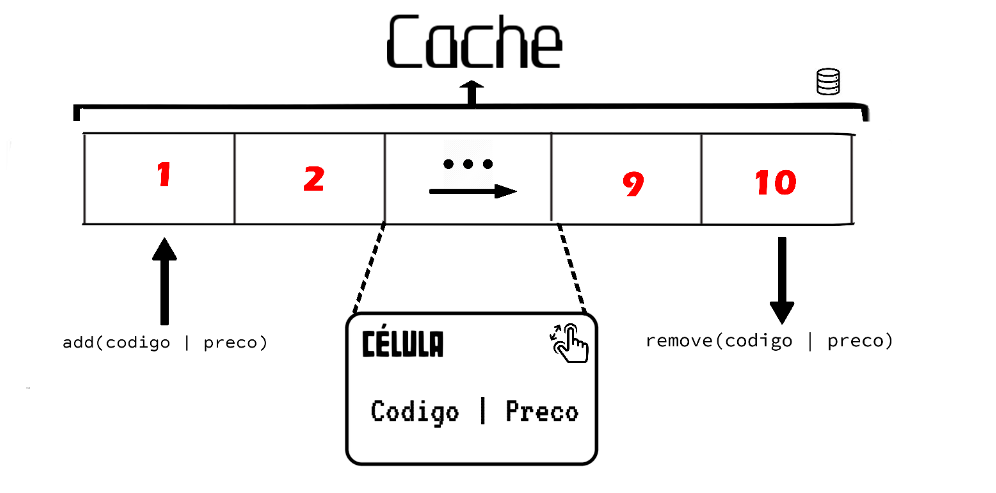
\includegraphics[scale=0.6]{cache.png}
    \label{img:htag}
    \caption{Cache de preços.}
\end{figure}

\begin{lstlisting}[language=C]
        struct celula {
        
        	int codigo;
        	int preco;
        
        };
      
        
        struct cache {
        
        	CELULA *cache;
        
        	int next;
        	int max;
        	int nr_elementos;
        };
        
\end{lstlisting}

%%IMAGEM CACHE
%%IMAGEM CACHE%%IMAGEM CACHE
%%IMAGEM CACHE%%IMAGEM CACHE%%IMAGEM CACHE
%%IMAGEM CACHE%%IMAGEM CACHE%%IMAGEM CACHE%%IMAGEM CACHE
%%IMAGEM CACHE%%IMAGEM CACHE%%IMAGEM CACHE%%IMAGEM CACHE%%IMAGEM CACHE

O algoritmo de gestão da cache, ou seja, de remoção de elementos é feito removendo o último elemento, ou seja, o primeiro de todos inserido visto que devido à aleatoridade dos pedidos de vendas não é muito relevante ter algoritmos especiais e/ou \textit{hashs} complicados, sendo que, um só será removido caso sejam introduzidos 10 novos códigos para a cache, mas, se um produto estiver a ser continuamente requisitado este não será removido. \par 

No nosso entender, não faz sentido ter \textit{counters} com o número de vezes que um código foi requisitado pois caso este deixe, por aleatoridade, de ser usado ficará na cache sem ser usado, ocupando um espaço importante \textbf{numa cache tão reduzida}.

Isto reduz assim o número de vezes que o servidor recorre aos ficheiros de dados, diminuindo operações custosas ao nivél do Sistema Operativo de \textit{buffering}, através de \textit{system calls} com operações de \textit{read} e \textit{write}.

\section{Agregação concorrente}

    Segue-se a representação referida anteriormente:

\begin{figure}[H]
    \centering
    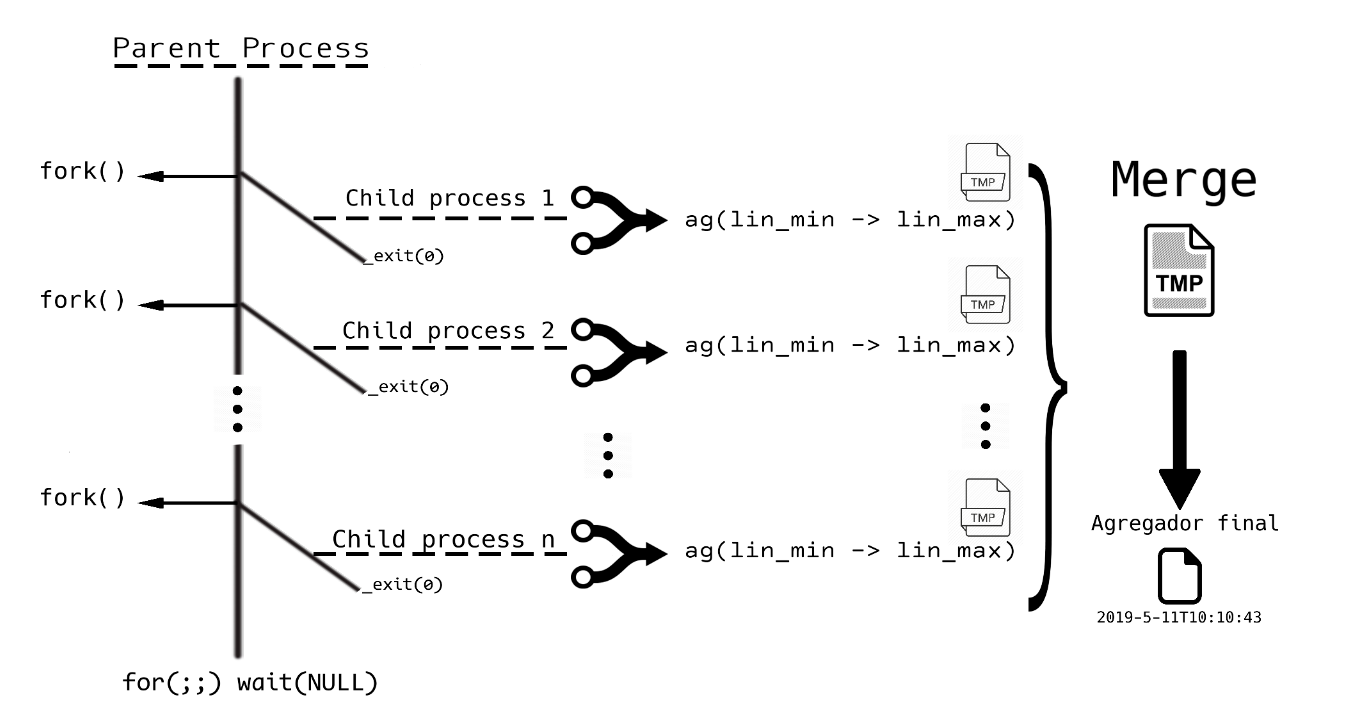
\includegraphics[scale=0.5]{agconc.png}
    \label{img:htag}
    \caption{Processo de agregação concorrente.}
\end{figure}


\section{Compactação do ficheiro STRINGS}

\hspace{0.50cm} A compactação deste ficheiro surge, de forma clara, devido à possibilidade de alteração de nomes de artigos na \textit{manutenção de artigos}. Com isto criam-se entradas \textbf{obsuletas} que podem ser perfeitamente compactadas. 

Para resolver este problema é importante esclarecer dois pontos: calcular a percentagem de \textbf{lixo} no STRINGS e \textbf{compactar}.

Para calcular a percentagem de lixo apenas dividimos o número de linhas do ficheiro ARTIGOS pelo número de linhas do ficheiro STRINGS, subtraímos por 1 e obtemos a percentagem requerida.

Ora o processo de compactação também é simples, começamos por renomear os ficheiros de ARTIGOS, STRINGS e STOCK para nomes temporários. De seguida cria-se ficheiros novos com os nomes originais. Percorremos o ARTIGOS e inserimos novamente a associação código <-> nome <-> preco utilizando as funções já definidas no programa \textbf{ma} que geram novas referências para os códigos.

Reconhece-se que se trata de uma solução não completamente dentro do mundo de Sistemas Operativos, mas consideramos que tiramos partido de performance e gestão de memória, visto que, após compactação todo o lixo é removido e não são criadas estruturas desnecessárias, como \textit{hashtables} ou \textit{linked lists} para armazenar tudo em memória.

\chapter{Notas relevantes}

\section{Compilação do projeto}

\hspace{0.50cm} Este projeto possui uma \textit{Makefile} presente no src/ que, conjuntamente com outras \textit{Makefile} secundárias, efetuam a compilação de todo o projeto, criação de diretorias onde serão armazenados ficheiros \textit{object} e \textit{linking} com estruturas \textbf{GLib} o que implica a pré-instalação destas bibliotecas.

\section{Bibliotecas implementadas}

\hspace{0.50cm} Como já foi referido anteriormente, todas as estruturas auxiliares, \textbf{cache}, \textbf{artigos}, constantes e \textit{paths} importantes encontram-se armazenadas na diretoria \textit{GLOBAL-SOURCE}, assim como a maior parte de funções auxiliares presentes nos programas implementados.

\section{\textit{Tracing} de erros e debugging}

\hspace{0.50cm} Este projeto revelou-se algo complicado a nivél de deteção de erros e \textit{debugging} e, de modo a facilitar isso mesmo, para além do \textit{report} dado pelo \textbf{stderr} o grupo efetuou um registo de todos os erros relativos a comandos inválidos, números \textit{out of range}, etc.. guardados no ficheiro "/FILES/ERRORLOG.log".

Segue-se uns exemplos de erros detetados:

\begin{lstlisting}[language=C]

    $cat ERRORLOG.log

    [./cv] client inserted an invalid command.
    [./ma] invalid command.
    [./cv] client requested code that does not exist.
    [./cv] client requested stock update to negative.
    ...
    
    <EOF>

\end{lstlisting}

\section{Sinais - aplicações neste projeto}

\hspace{0.5cm} Existem algumas aplicações de sinais durante o código, nomeadamente, pelo servidor. 

Acontece aquando a terminação do processo do servidor quando este recebe um SIGINT e, ao invés de morrer de imediato, "arruma a casa", isto é, elimina todos os ficheiros desnecessários/temporários, registos de clientes \textit{"loggados"} e termina o processo de todos os clientes que possam estar ligados ao servidor, enviando um sinal para os mesmos (um SIGINT também).



\chapter{Considerações finais}

\hspace{0.50cm} Este projeto descreve uma extrema importância no olhar que todos os programadores devem ter acerca do mundo \textit{Out-of-core} que aparentemente é mais relevante do que saber escrever umas linhas de código. \par

A noção de como é feita a gestão de memória e de procesos foi crucial na perceção e atenção no código que pode ser escrito e na noção que apesar de tudo, nada é garantido, por exemplo, a partir de um simples \textit{printf(...)}.

Podia ter sido melhor considerados fatores de segurança devido a permissão de ficheiros para utilização/alteração/remoção e podia ter sido economizada memória em certas operações.

Existem \textit{writes} no \textit{stdin} presentes no servidor/cliente desnecessários, usados para o utilizador do sistema ter a noção da existência de uma cache, de pedidos ao servidor para atualizar precos, stocks, entre outros.

Apesar de tudo, o grupo considera que o \textit{core} do trabalho foi implementado com sucesso e responde de uma forma correta a todas as questões propostas.

\end{document}














